\documentclass{article}
\usepackage[top=3cm,bottom=3cm,right=3cm,left=3cm]{geometry}
\usepackage[francais]{babel}
\usepackage[utf8]{inputenc}
%\usepackage[latin1]{inputenc}
\usepackage[T1]{fontenc}
\usepackage[absolute]{textpos} 
\usepackage{graphicx}

\title{Rapport du projet : Une ligne de produits logiciels pour la réalisation de jeux d'arcades}


\begin{document}

\def\blurb{%
  Université des Sciences de Montpellier \\
  Master 1 Semestre 2 \\
  Unité d'Enseignement TER \\
  Site Internet : http://code.google.com/p/mus-d/}
\def\clap#1{\hbox to 0pt{\hss #1\hss}}%
\def\ligne#1{%
  \hbox to \hsize{%
    \vbox{\centering #1}}}%
\def\haut#1#2#3{%
  \hbox to \hsize{%
    \rlap{\vtop{\raggedright #1}}%
    \hss
    \clap{\vtop{\centering #2}}%
    \hss
    \llap{\vtop{\raggedleft #3}}}}%
\def\bas#1#2#3{%
  \hbox to \hsize{%
    \rlap{\vbox{\raggedright #1}}%
    \hss
    \clap{\vbox{\centering #2}}%
    \hss
    \llap{\vbox{\raggedleft #3}}}}%
\begin{document}
\thispagestyle{empty}\vbox to .9\vsize{%
  \vss
  \vbox to 1\vsize{%
    \haut{}{\blurb}{}
    \vfill
    \ligne{\Large \maketitle{}}
    \vfill
    \ligne{%
      \begin{tabular}{l}
	Jonathan \textsc{Fhal} \\
        Mélanie \textsc{König} \\
        Laurent \textsc{Maillet} \\
        Romain \textsc{Maneschi} (chef) \\
        Audrey \textsc{Novak}
      \end{tabular}
      }
    }%
  \vss
  }

\newpage

\tableofcontents

\newpage

\section{Objectif du sujet}
	\subsection{Présentation du sujet :}
	Ce projet est réalisé dans le cadre de l'unité d'enseignement TER, en première année de Master Informatique à l'université des Sciences de Montpellier.
	\indent Il consiste à créer un ensemble de classes qui permettra de programmer plus facilement des jeux de type "arcade". Ces jeux pourront être utilisés sur Internet, quelque soit le navigateur et le système d'exploitation de l'utilisateur. En outre ils pourront également tourner directement dans le système de l'utilisateur.
	\subsection{Définitions :}
	\subsubsection{Bibliothèque Logicielle}
		Egalement appelée librairie, une bibliothèque est constituée d'un ensemble de fonctions qui pourront être réutilisées sans avoir à les réécrire. Ces fonctions sont la plupart du temps regroupées par thèmes.

	\subsubsection{Ligne de produits}
		Une ligne de produits est un ensemble de produits mis à disposition par une entreprise pour répondre à un même besoin, ou ayant des caractèristiques communes. Elle permet également d'augmenter la productivité tout en diminuant le temps et donc le coût de réalisation du produit. \\ \\
		\indent \textbf{Ligne de produits logiciels} \\
			\indent Ensemble de logiciels appartenant à un domaine particulier, ici la création de jeux d'arcades. En informatique une ligne de produits est également appelée un framework. Généralement, un framework est codé dans un langage objet, par conséquent il est composé d'une classe mère de laquelle découle plusieurs classes filles. Ainsi un programmeur doit réimplémenter les classes qui l'intéressent pour créer son logiciel. \\
			\indent Une ligne de produits logiciels est une surcouche des bibliothèques et permet donc, non seulement de pouvoir réutiliser du code mais aussi et surtout de donner une architecture précise aux logiciels qui l'utilisent. De plus un framework doit être nécessairement extensible pour s'adapter à un plus grand nombre de logiciels.
	\subsubsection{Jeux d'Arcades}
		Les jeux d'arcades sont principalement des jeux à deux dimensions. La jouabilité est très simple ce qui rend ce type de jeux très populaires. Il n'y a généralement pas d'intelligence artificielle (ou très peu évoluée) et encore moins de parties réseaux (les joueurs s'affrontent sur la même machine). \\
		\indent A l'origine ce type de jeux à été créé pour les salles de jeux ou certains bars, c'est pour cela que le niveau du jeu est exponentiel, afin que le joueur remette en permanence de l'argent pour faire vivre son personnage. Ceci explique aussi le fait qu'il n'y ait pas de sauvegardes des parties. \\
		\indent Quelques exemples de jeux bien connus : Pac-Man, Casse-Briques, Ping-pong...

\section{Fonctionnalités}
	Grâce à notre framework, un programmeur pourra aisément coder les comportements les plus utilisés dans les jeux de type arcade. Ces comportements sont les suivants : collision (rebond, explosion), scène de jeu fermée ou ouverte (les objets qui sortent à un coin réapparaissent à l'autre). De plus, il nous a paru nécessaire de faciliter un maximum les opérations de drag et drop afin que le programmeur du jeu puisse les utiliser plus simplement. Nous avons également choisi d'implémenter des classes utiles, permettant par exemple de mélanger un tableau ou d'utiliser un timer. \\
	\indent Pour tester la fiabilité de notre framework et donner quelques exemples de code à nos utilisateurs, nous programmerons un jeu de ping-pong et un jeu de pac-man. \\
	\indent De plus, pour faciliter la création de jeux, nous proposerons un créateur de jeux, ainsi, par simple glissement d'objets l'utilisateur pourra créer des jeux ou créer ses propres niveaux. Toutes les opérations réalisées avec ce logiciel seront transcrites en code, l'utilisateur n'aura qu'à compiler ce code pour obtenir son jeu.

\section{Contraintes}
	La principale contrainte est que nos jeux doivent être jouables sur internet et sur tous types de système d'exploitation.  De plus, nos application seront également capables de tourner en dehors d'un explorateur internet. \\
\indent Enfin, nous avons décidé d'implémenter nos classes sous la forme du modèle MVC (Model Controler View).

\section{Organisation}
	\subsection{Répartition des tâches}
		La répartition des tâches s'est éffectuée selon les préférences de chacun.
		\begin{itemize}
			\item Maneschi Romain (chef de groupe) : Coeur du projet (partie graphique)
			\item Maillet Laurent : Coeur du projet (partie interne)
			\item Novak Audrey : Créateur de jeux
			\item Fhal Jonathan : Créations de 2 ou 3 jeux utilisant le framework
			\item König Mélanie : Coeur du projet (partie algorithmique)
	\subsection{Diagramme de Gantt}
		Nous prévoyons de suivre cette ligne de conduite :
		\begin{center}
			\begin{textblock*}{19cm}(1.5cm,16cm) 
				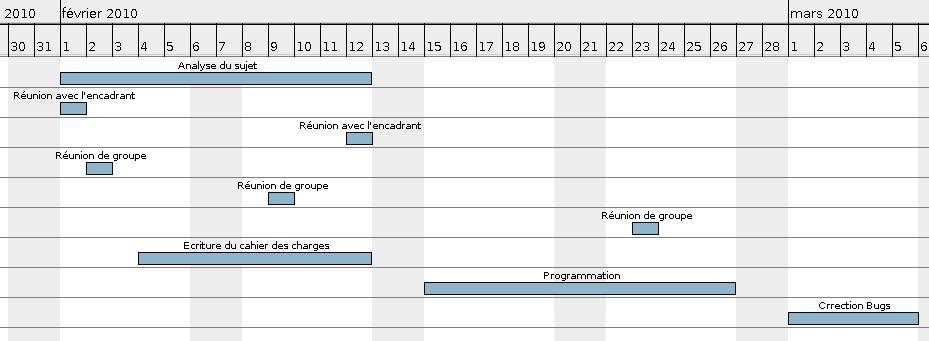
\includegraphics[width=1.00\textwidth]{diagramme-gantt.jpg}
			\end{textblock*}		
		\end{center}
\newpage
\section{Convention de nommage}
		\indent Nous avons fait le choix de programmer en français. Toutes nos classes et interfaces seront préfixées par un M, afin d'éviter les collisions de noms avec d'autres framework. Le M représente notre nom de groupe (MUS-D).
		\ident De plus nous utiliserons la syntaxe suivante :
		\begin{itemize}
			\item MClasse : majuscule puis minuscule et majuscule pour séparer les mots.
			\item MIInterface : même syntaxe que les classes, mais précédée d'un I.
			\item méthodeDeClasse : minuscule puis majuscule pour séparer les mots.
			\item attribut\_de\_classe : minuscule puis underscore pour séparer les mots.
		\end{itemize}
		
	\subsection{Commentaires}
		\indent Comme nous créons une ligne de produits logiciels, nous nous devons d'être rigoureux sur les commentaires de notre code afin que les futurs utilisateurs comprennent notre façon de programmer et donc la manière dont il devront programmer leurs applications.
		\indent Pour se faire nous utiliserons asDoc, une application permettant de créer des pages HTML à partir de balises placées dans notre code. Ce logiciel est distribué de base avec Flex Builder, le plugin eclipse permettant de programmer facilement en flex et donc en action script.

\section{Outils de travail}
	\subsection{Choix du langage}
		\indent Ce projet impose de pouvoir utiliser cette ligne de produits pour créer nos propres jeux d'arcades. Ces jeux doivent être jouables sur Internet. De nos jours il n'existe pas beaucoup de langages de programmation permettant cela. Les deux plus répandus sont JavaScript et Flex. Flex étant un tout nouveau langage développé par Adobe, il nous à paru interressant de le découvrir et d'exploiter sa richesse plutôt que de réutiliser un langage connu de tous : JavaScript.
		\subsubsection{ActionScript}
			\indent L'ActionScript est le langage propriétaire d'Adobe, développé dans le but de contrer JavaScript. La syntaxe est très proche de JavaScript et permet de faire des applications orientées objet.
		\subsubsection{Flex}
			\indent Ce nouveau langage basé sur ActionScript permet de créer des clients internets riches avec une syntaxe à balises. Ainsi les scripts écrits en Flex sont transformés en ActionScript puis compilés en SWF (format propriétaire d'Adobe également appelé Flash). Ainsi tout navigateur équipé de Flash peut lire les applications Flex.
			\ident Nous créerons donc notre framework en ActionScript, car c'est un langage objet, actuellement en version 3 (donc stable et évolué). Cela laisse donc le choix aux utilisateurs de notre framework de réimplémenter nos classes en ActionScript ou de développer directement leurs applications en Flex.
			\ident L'inconvénient de ce choix est que toute la technologie est propriétaire. Il faudra donc que l'utilisateur final ait tous les outils nécessaires à la programmation et surtout compilation de Flex.
	\subsection{IDE}
		\indent Adobe a fait le choix de ne pas développer d'IDE spécialisé pour son langage, préférant utiliser Eclipse par le biais d'un plugin. Eclipse est un IDE très populaire car libre de droit et très performant puisqu'en version 3. Nous ne sommes donc pas perdus puisque nous avons l'habitude de développer avec cet IDE.
	\subsection{Google Code}
		\indent Pour pouvoir travailler en groupe nous avons besoin d'un site internet pour regrouper nos codes et nos idées. Google Code est une plate-forme nous offrant un Wiki pour échanger nos idées, un serveur SVN pour partager nos sources, un espace de stockage de fichiers et enfin un contrôleur de bugs afin d'être prévenu d'éventuels problèmes.
		\ident De plus il est entièrement gratuit et est hébergé chez Google, ce qui nous assure une plus grande sérénité quand à la sauvegarde de nos données.
	\subsection{SVN}
		\indent Puisque Google nous offre généreusement un serveur SVN nous l'utiliserons pour garder la même version pour chacun des développeurs. 
		\ident Sous Linux nous utiliserons le client RapidSvn pour sa simplicité (un tutorial sur son utilisation est disponible sur le site du projet).
		\ident Sous Windows nous utiliserons Tortoise pour les mêmes raisons.


\end{document}
